\documentclass[12pt]{article}
%\usepackage[T1]{fontenc}
%\usepackage[latin9]{inputenc}
\usepackage[margin=1in]{geometry}

% To compile in Times New Roman, use the following two lines.
% You'll need to compile with xelatex or lualatex.
% If you don't have these compilers, you can outcomment these two lines,
% but it won't be in Times New Roman.
\usepackage{fontspec}
%\setmainfont{Times New Roman}

\usepackage{sectsty} % to get the section headings to be smaller
\usepackage{natbib}
\usepackage{bbm}
\usepackage{amsmath,amssymb,amsthm,mathtools}
\usepackage{caption}
\usepackage{algorithmic}
\usepackage{authblk} % if you are using texlive on macports, install texlive-latex-extra to get this

% Uses the sectsty package to make section headings smaller.
\sectionfont{\fontsize{12}{15}\selectfont}
\subsectionfont{\fontsize{12}{15}\selectfont}

\newcommand{\Prob}{\mathbb{P}}
\newcommand{\E}{\mathbb{E}}
\newcommand{\EI}{\mathrm{EI}}
\newcommand{\Dir}{\mathrm{Dirichlet}}
\newcommand{\PI}{\text{P}^*}
\newcommand{\mb}{\mathbf}
\newtheorem{Algorithm}{Algorithm}
\newtheorem{theorem}{Theorem}
\newtheorem{lemma}{Lemma}
\newtheorem{proposition}{Proposition}
\newtheorem{remark}{Remark}

\begin{document}

\title{Peptide Optimization by OptimalLearning (POOL): Identification and refinement of peptides for reversible chemoenzymatic labeling}

\author[1]{Jialei Wang}
\author[2]{Michael D. Burkart}
\author[1]{Peter I. Frazier}
\author[2]{Nathan Gianneschi}
\author[3]{Michael K. Gilson}
\author[4]{Nicholas Kosa}
\author[2]{Lorillee Tallorin} % Lori's full name has two ll's in it.
\author[1]{Pu Yang\thanks{Author order is alphabetical, except for first author Jialei Wang.}}

\affil[1]{School of Operations Research \& Information Engineering, Cornell University}
\affil[2]{Department of Chemistry and Biochemistry, UC San Diego}
\affil[3]{Skaggs School of Pharmacy and Pharmaceutical Sciences, UC San D}
\affil[4]{Bioo Scientific Corp, Austin TX} %, \URL{}}

%\affil[1]{School of Operations Research \& Information Engineering, Cornell University, Ithaca, NY 14853}
%\affil[2]{Department of Chemistry and Biochemistry, University of California, San Diego, La Jolla, CA 92093}
%\affil[3]{Skaggs School of Pharmacy and Pharmaceutical Sciences, University of California, San Diego, La Jolla, CA 92093}
%\affil[4]{Bioo Scientific Corp, Austin, TX 78744} %, \URL{}}


%\EMAIL{mburkart@ucsd.edu}, \EMAIL{ngianneschi@ucsd.edu}, \EMAIL{ltallorin@ucsd.edu}, \EMAIL{mgilson@ucsd.edu}}

\date{\vspace{-5ex}} % Remove the date, and the space it takes

\maketitle


\abstract{%
We consider a Bayesian active learning problem arising in biochemistry, in which we wish to find a peptide that (1) has a certain expensive-to-ascertain biochemical property (it is a substrate for two protein-modifying enzymes, phosphopantetheinyltransferase and ACP hydrolase); and (2) is as short as possible.
Finding such a peptide would allow tracking protein interactions with great ease, and would support a number of innovations in medicine, biochemistry, and materials science.
However, such peptides are difficult to find, because the set of peptides is large, only a small fraction have the desired property, and ascertaining whether or not a peptide has the desired property requires performing a time-consuming laboratory experiment.
We present a machine learning method for choosing which peptides to test to find such a peptide as quickly as possible. 
We prove theoretical bounds on its solution quality, 
demonstrate in simulation that it outperforms two natural benchmark methods, 
and then describe how it was used in practice to find a peptide with the desired property that is shorter than the shortest previously known.
While our method was developed for this specific application in biochemistry, it can also be used in other Bayesian active learning problems in which we wish to find an exemplar whose expensive-to-obtain binary label is positive, and for which a secondary easy-to-evaluate cost objective is as small as possible. 
% Enter your abstract
}%

% Sample
%\KEYWORDS{deterministic inventory theory; infinite linear programming duality;
%  existence of optimal policies; semi-Markov decision process; cyclic schedule}

% Fill in data. If unknown, outcomment the field
% \KEYWORDS{Bayesian, Active Learning, Naive Bayes} 

\section{Introduction}

In this paper, we use machine learning to address a specific instance of a problem common in medicine, materials science, chemistry, and other physical sciences.  In this class of problems, we wish to find a molecule with a particular biological or chemical property. While we have historical data on related molecules or related properties that can support predictive modeling, the only way that we can determine with certainty whether a particular molecule has the property of interest (in colloquial language, ``is a hit'') is to synthesize and test it in a time-consuming laboratory experiment. Success is hampered by the enormous search space, and the limits imposed by experimental cost on the number of molecules that can be tested.  Within this context, we wish to use mathematical methods to recommend which experiments to perform, so as to reliably find a hit within a given experimental budget. Common examples include drug discovery, in which we wish to find a molecule that can be effective in treating a particular disease \citep{Negoescu2010}, and materials discovery \citep{material1, material2}, in which we wish to find a molecule that has a particular physical or chemical property.

The instance of this problem that we consider in detail in this paper comes from biochemistry: we wish to find a peptide that is (1) as short as possible; and (2) is a substrate for two protein-modifying enzymes, phosphopantetheinyltransferase (PPTase) and ACP hydrolase (AcpH). These protein-modifying enzymes can be used to attach and detach arbitrary molecules to their substrates.  In particular, 
 as shown in Figure \ref{fig:labeling}, 
we can use PPTase to attach a fluorescent ``tag'' or ``label'' to peptides that we would discover that are substrates for both enzymes, allowing us to track the peptide, starting from a time of our choosing.  We can then use AcpH to remove the fluorescent tag at a time of our choosing, and this reversible process is shown in Figure \ref{fig:reversible}.  If this peptide were short, then it could be inserted into a protein or peptide-based catalytic complex of our choosing without disrupting its activity, allowing monitoring of biological and catalytic systems.  This monitoring tool would have a number of applications in medicine, biology, and materials science \citep{nick}.


\begin{figure}[hpt] 
\center
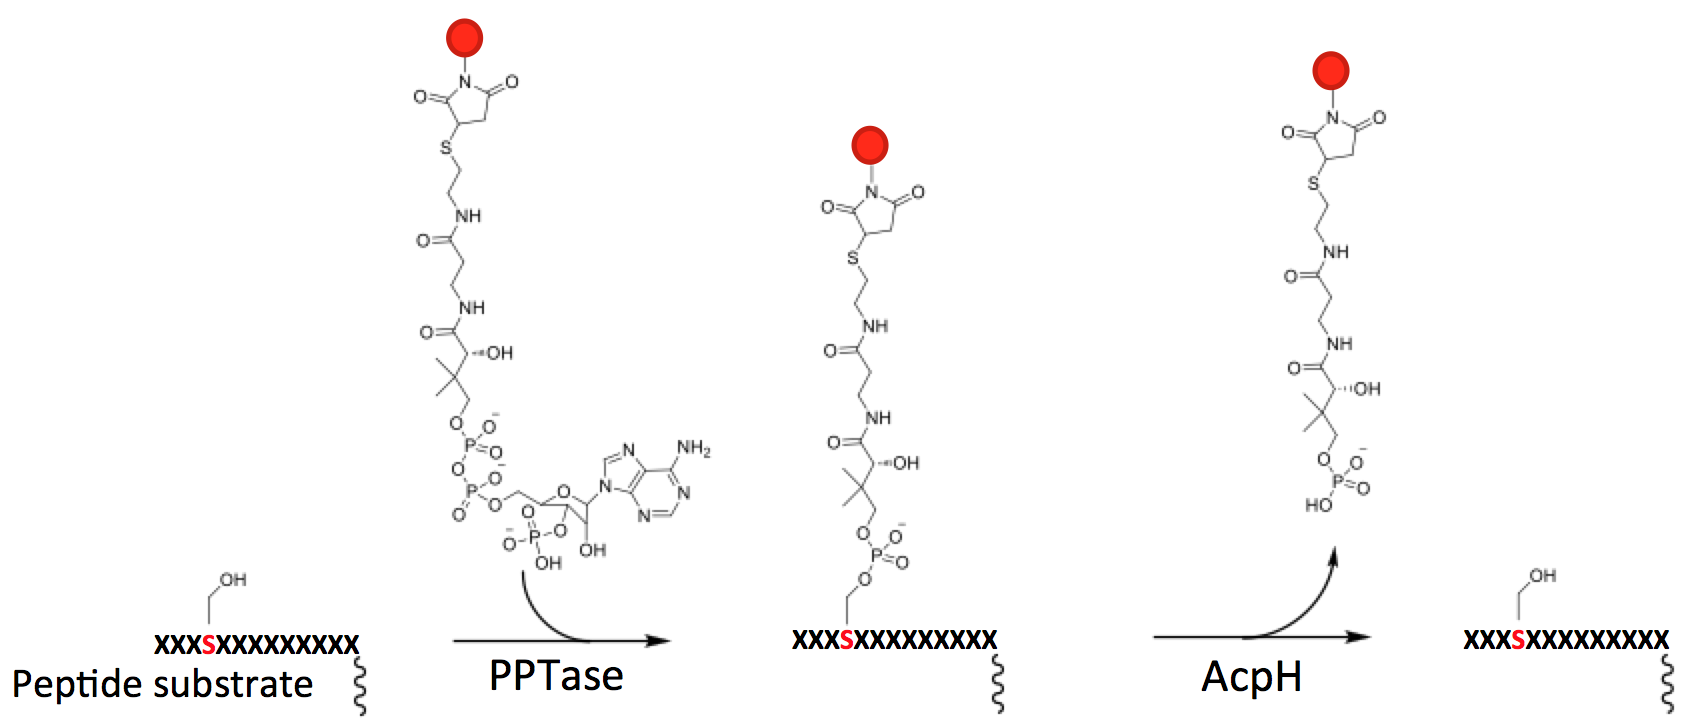
\includegraphics[width=\textwidth]{pic/labeling.png}
\caption{ Peptide labeling and unlabeling}
\label{fig:labeling}
\end{figure}

\begin{figure}[hpt] 
\center
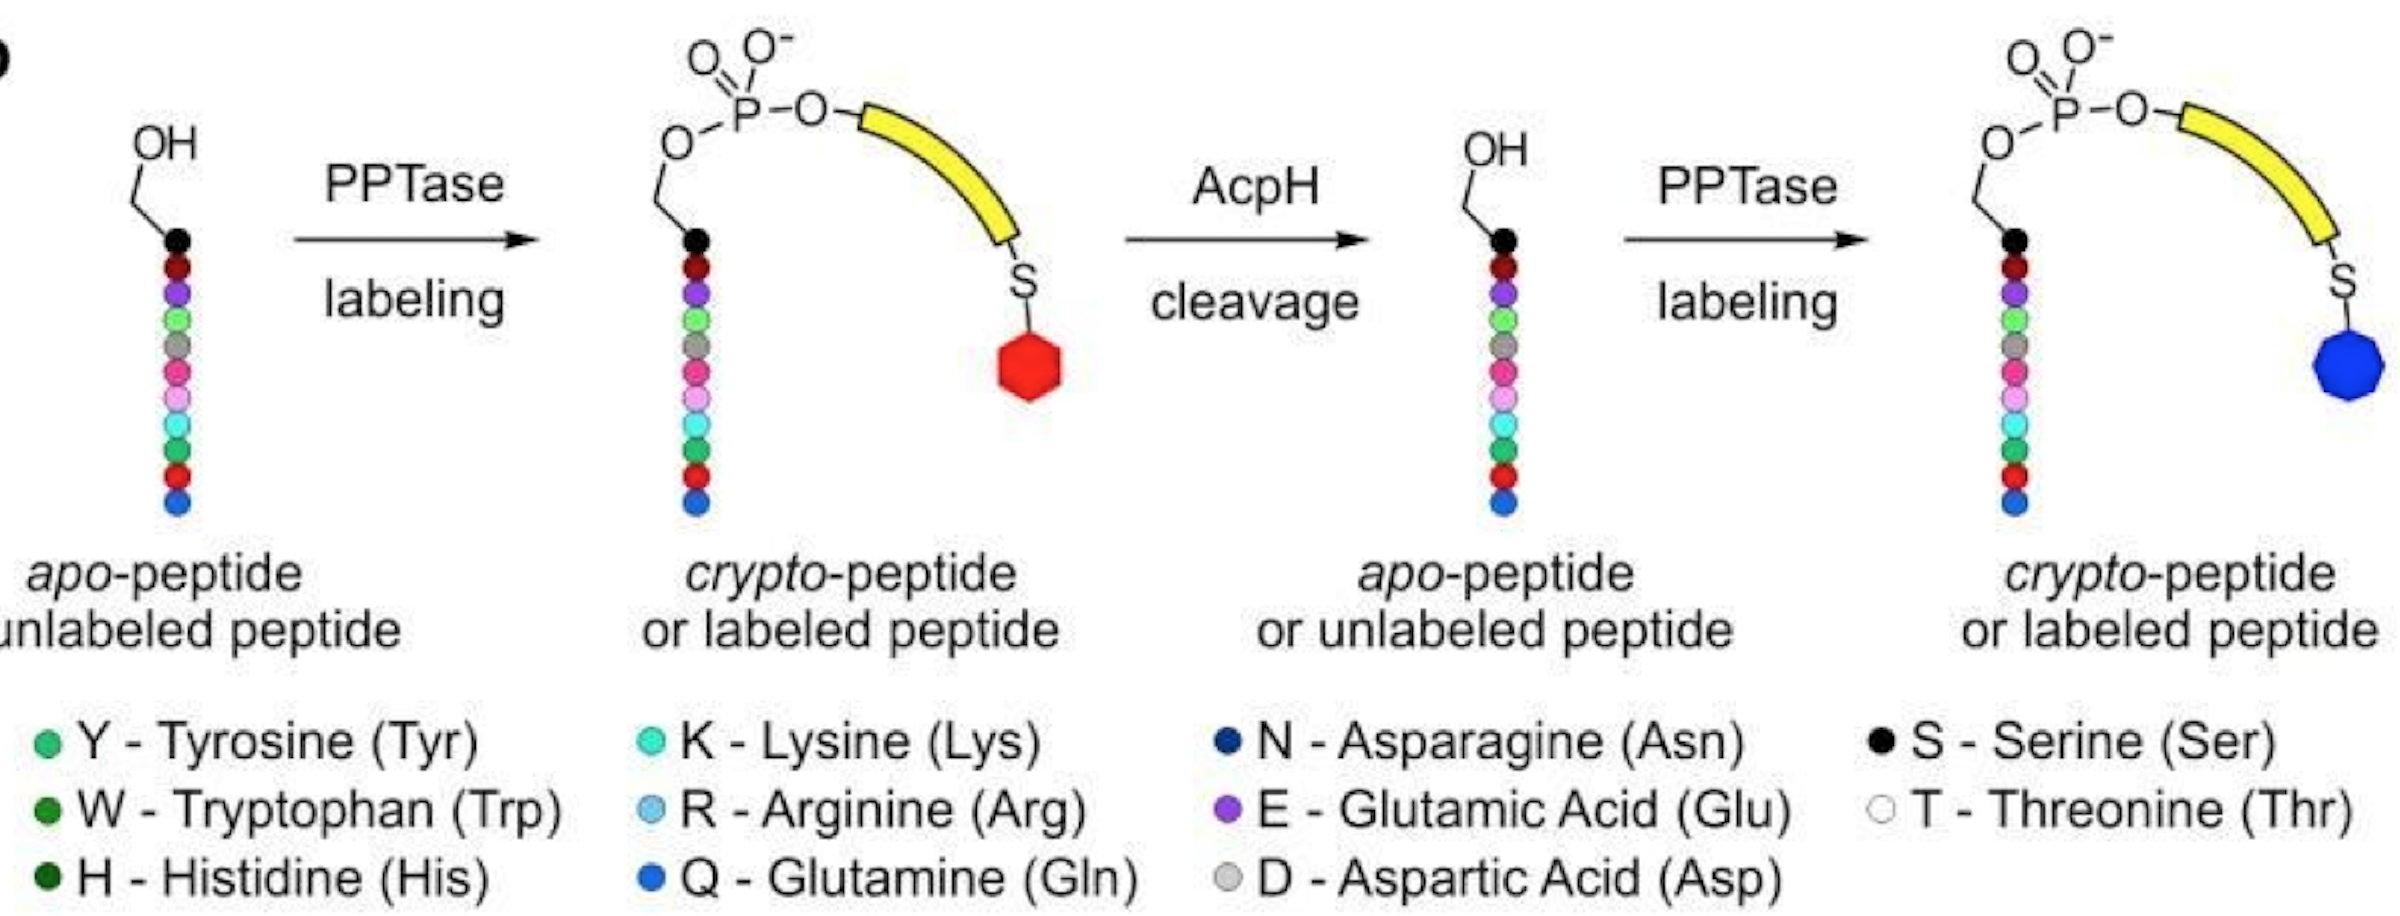
\includegraphics[width=\textwidth]{pic/reversible_peptide.png}
\caption{ Illustration of the reversible process}
\label{fig:reversible}
\end{figure}
Finding such a peptide is challenging, because the number of peptides is large, and only a small fraction of them are substrates for both enzymes (i.e., are ``hits'').  A peptide is a string of amino acids, of which 20 occur in nature, so there are $20^n$ peptides of length $n$.  The typical length of the peptides under consideration is 15 amino acids long, and the number of peptides with length 15 is $20^{15} \approx 3.3 \times 10^{19}$.  Of these, we estimate that approximately $1$ in $10^4$ is a substrate. We can test peptides in batches of size approximately $300$, and each batch requires approximately one week of work, several thousand dollars in materials, and access to an expensive shared machine on which time can be reserved for a batch of experiments approximately once every two months. If we were to test peptides of length $15$ uniformly at random, then we would need to test $n = \log(1/2) / \log(1-10^{-4}) \approx 6931$ peptides to ensure a probability of $1/2$ of finding at least one hit, which would in turn require 23 batches of experiments, and roughly four years' time.

% Prob(at least one hit in n)
% = 1 - Prob(no hits in n) 
% = 1 - Prob(no hit in 1)^n
% = 1 - (1 - Prob(hit in n))^n
% = 1 - (1 - 10^{-4})^n
% Solve for this being equal to 1/2, get 
% n = log(1/2) / log(1-10^{-4})

% PF: I am leaving out some of the ideas in this paragraph.  We can tell these ideas in the experimental section.

% There are two current approaches: One is to search peptides without quantitive help, and purely based on domain knowledge. This is likely to fail because the number of peptides with the desired property is small, and there is no clear direction to find minimal peptide with desired property. The other approach is to use available data to train a statistical model, and test the top N most likely hits and then stop. However, considering the small size of training set compared with the huge search space, the trained statistical model only has ``local'' knowledge while lack information about the rest part of the space, and this approach will only find local optimum.

% If we want to talk more about existing techniques, we could also describe phage display.

To address this challenge, we formulate this problem as a Bayesian active learning problem.  We first develop a Bayesian classification method, which combines Naive Bayes \citep{NB}, a prior distribution encoding knowledge from domain experts, and training data from naturally occurring and longer peptide substrates, to predict whether a short peptide is a hit. We then use the joint probability distributed over unobserved labels (``hit'' or ``miss'') of all peptides created by this classification method within a combinatorial optimization framework to find a {\it set} of peptides to test that, when taken together, are most likely to produce a hit.  We provide a theoretical performance guarantee on the quality of the resulting set of peptides to test, and using simulation, we show that this combination of prediction and optimization provides robust results that are better than a more naive use of the predictive model that considers only marginal probabilities, and a benchmark method of truncating and mutating known hits at random. We then describe laboratory results in which this method was used to discover peptide substrates that are shorter than the shortest previously known: the ybbR sequence \citep{ybbr}.


% The accuracy of this classification model is, however, too low to simply take the single peptide most likely to be a hit, or even the top 300 most likely to be a hit, and have it provide reliable results. We then use combinatorial optimization to post-process the output of this classification method to find a set of peptides to test that, when taken together, are most likely to produce a hit.  We show that this method provides robust results that are better than more naive use of the predictive model

While the methods we develop were designed to address a particular problem arising in biochemistry, the formal model we propose is general, and can be used whenever we have a large collection of exemplars with expensive-to-obtain labels, and we wish to choose exemplars to evaluate so as to find one with both a positive label and a small secondary cost objective, within a limited budget.

This paper builds on a number of recently developed methods for optimal search, all of which aim to effectively collect information so as to make the best decisions under uncertainty. In this setting, they need to trade off the reward by sampling (i.e. exploitation) and the cost by acquiring this information (i.e. exploration). There are a number of methods in the similar setting proposed in the active learning research community in the past a few years. For example, in document recommendation system, a new model quality measure that quantatively manage trade-off between expoitation and exploration \citep{filter} was proposed. In information retrevial, there are a few papers about batch mode (parallel sampling) active learning in various contexts \citep{Chen2013, Hoi2006, Hoi2006a}, although they only aim to maximize information gain (i.e. pure exploration).

%For example, in drug discovery, people search for a chemical derivative of the base molecule that best treats disease. To achieve this goal, they choose molecules to test to maximize the expected quality of the
%best compound discovered \citep{Negoescu2010}. Since the budget for testing is limited, they need to test the most informative and high quality molecules. To address this problem, there are a number of methods have been proposed by other research groups: in active learning research community, Golovin, Krause \& Ray Jones \& Schonlau proposed Expected Improvement algorithm to sample points sequentially \citep{Jones1998}. Ginsbourger used constant liar heuristic to extend Expected Improvement algorithm to parallel setting \citep{Ginsbourger2008}. There are quite a few papers about parallel sampling in active learning research
%community \citep{Chen2013, Hoi2006, Hoi2006a} , but they only aim to maximize information gain (i.e. pure exploration).

In section 2, we provide a formal model of our problem.  In section 3, we state the Bayesian classification model used for the problem. In section 4, we provide the formulation of the proposed optimization algorithm, prove its performance guarantee, and summarize the algorithm in pseudo code. In section 5, we use available real data to validate our statistical model, compare the performance of our proposed optimization method against
other methods, and show progress of this biochemical application using our method.

\section{Problem Formulation} \label{sec:problem}

We now formulate our applied problem as an active learning problem.  
Let $E$ be a generic space of exemplars.  In our application, $E$ is the space of peptides. Each element $x \in E$ has an unknown binary label $y(x)=\{0,1\}$.  In our application, $y(x)$ is 1 if $x$ is a hit, i.e., is a substrate for both enzymes, and 0 if not.
A known deterministic function $f(x)$ measures the cost or disutility associated with $x$.  In our application, $f(x)$ is the length of the peptide, as longer peptides interfere more with the system being monitored. Our goal is to perform experiments so as to find $x$ with a positive label and a cost $f(x)$ that is as small as possible.

To obtain labels of exemplars, we can do experiments in batches, which evaluate the labels for a subset $S \subseteq E$. The cardinality of $S$ is constrained by some $K$ (i.e. $|S| \leq K$), modeling our budget for performing experiments. We measure the quality of $S$ by 
\begin{equation} \label{eq:fS}
f^*(S)= \underset{x \in S:y(x)=1}{\min} f(x),
\end{equation}
where we assume $\min \emptyset = \infty$. $f^*(S)$ measures the smallest cost function for positive labeled elements in the set $S$, and in our application, that means the shortest length of desired peptides in the set of peptides to test.


Let $b$ be a target value and we wish to find $S\subseteq E$ such that $f^*(S)$ is better than $b$. In our application, we let $b$ be the length of the shortest previously known desired peptide. $f^*(S)$ is unknown because we do not know the label $y(x)$ for $x \in S$ yet. We assume a joint probability distribution over $y(x): x \in E$, which is determined by the underlying statistical model for a particular problem, and for our application, the model is described in Section \ref{sec:stat model}. Based on the probability distribution we consider the following two quality measures for $S$:
\begin{equation} \label{eq:twomeasure}
  \begin{aligned}
    &\text{Probability of Improvement: }&\PI(S) = \mathbb{P}(f^*(S) < b)\\
    &\text{Expected Improvement: }&\EI(S) = \E [(b-f^*(S))^+]
  \end{aligned}
\end{equation}
Given constraint on the cardinality of $S$, we wish to find $S$ that maximizes one of these two measures. Let $g(S)$ be either $\PI(S)$ or $\EI(S)$, and we can write our goal as

\begin{equation}
  \max_{S \subseteq E: |S| \leq K} g(S). 
  \label{eq:opt}
\end{equation}

\section{Statistical model} \label{sec:stat model}
To construct the joint probability distribution over $y(x): x \in E$, which is needed to calculate \eqref{eq:twomeasure} and to choose which peptides to test, we develop a Bayesian classification method for our application, which combines Naive Bayes and a prior distribution encoding knowledge from domain experts. Let $X=(X_1,\ldots,X_n)$ be an instance with $n$ features and $Y$ be its label. Using Bayes's Rule, we have:

\begin{equation*}
\Prob(Y=y|X=x)=\frac{\Prob(X=x|Y=y)\Prob(Y=y)}{\Prob(X=x)}=\frac{\Prob(X=x|Y=y)\Prob(Y=y)}{\sum_{y'}\Prob(X=x|Y=y')\Prob(Y=y')}
\end{equation*}

The Naive Bayes classifier assumes that the presence or absence of a particular feature is unrelated to the presence or absence of any other feature, given the class variable, i.e.

\begin{equation*}
\Prob(Y=y|X=x) = \frac{\prod_{j=1}^n\Prob(X_j=x_j|Y=y)\Prob(Y=y)}{\sum_{y'}\prod_{j=1}^n\Prob(X_j=x_j|Y=y)\Prob(Y=y)}
\end{equation*}

In our application, we have a set of peptides, each with length less than or equal to $L$. Each peptide is a sequence of amino acids. We use a reduced alphabet for amino-acids, i.e., we group them into $K$ groups. For each peptide, let $A_i$ be the amino acid on position $j$, and let $X_i$ be the class of this amino acid. For a specific enzyme, let $Y(x)=1$ if peptide $x$ is a substrate for that enzyme and 0 if not.

We let $\theta_{y,j}(k)=\Prob(X_i=k|Y(X)=y)$, for each $j=1,\ldots,L$, $k=1,\ldots,K$ and $y\in\{0,1\}$. We further assume some known prior distribution $\Prob(Y(x)=y)$, $y\in\{0,1\}$. Let $\theta$ be the full set of parameters $\theta_{y,j}(k)$, for $j=1,\ldots,L$, $k=1,\ldots,K$ and $y\in\{0,1\}$. Then, given an unlabeled peptide, we can calculate its probability of being a substrate as:

\begin{equation} \label{eq:model}
  \Prob\left(Y(x) = 1 | \theta\right) =
  \frac{\Prob(Y(x)=1) \prod_{j} \theta_{1,j}(x_j)}{
  \left[ \Prob(Y(x)=1) \prod_{j} \theta_{1,j}(x_j)\right] +
  \left[ \Prob(Y(x)=0) \prod_{j} \theta_{0,j}(x_j)\right]}
\end{equation}

We estimate the parameters $\theta_{y,j}(k)$ using Bayesian inference. We assume for each $j=1,\ldots,L$, $y\in\{0,1\}$, the vector $\theta_{y,j}\sim\Dir(\alpha_{y,j}(1),\ldots,\alpha_{y,j}(K))$. A good initial choice for the parameter vector $\alpha_{y,j} = (\alpha_{y,j}(1),\ldots,\alpha_{y,j}(6))$ can be choosing $\alpha_{y,j}(k)$ to be constant across $k$, and $y$, and to only depend upon $j$. Since amino acids further from the serine are less likely to have a strong influence on its activity, we choose this value to be $1$ in the positions next to the serine and to increase as $j$ moves further.

We further assume two hyper parameters $\gamma_0$ and $\gamma_1$ that characterize the distribution for $y=0$ and $y=1$ respectively. Then, with the prior distribution and hyper parameters, our posterior distribution is also Dirichlet. In particular, it is 
$\Dir( \alpha_{y,j}(1) + \gamma_yN_{y,j}(1), \ldots, \alpha_{y,j}(K) + \gamma_yN_{y,j}(K))$,
where $N_{y,j}(k)$ counts how many peptides $x$ in the training data with $Y(x)=y$ had $x_j=k$.  That is, it counts how many peptides had amino acid $j$ in class $j$.

Since our training data is expensive and highly skewed, we use the leave-one-out cross validation procedure to choose the optimal hyper parameters. For each setting of the hyper parameters, we obtain an receiver operating characteristic(ROC) curve using the result of the leave-one out procedure and choose the setting with highest AUC(area under curve).

%[Put two ROC curves here, one for leave-one-out and one for using the 1st data set as training and 2nd data set as test, to be continued ...]

\begin{figure}[hpt] 
\center
\begin{minipage}[b]{0.45\linewidth}
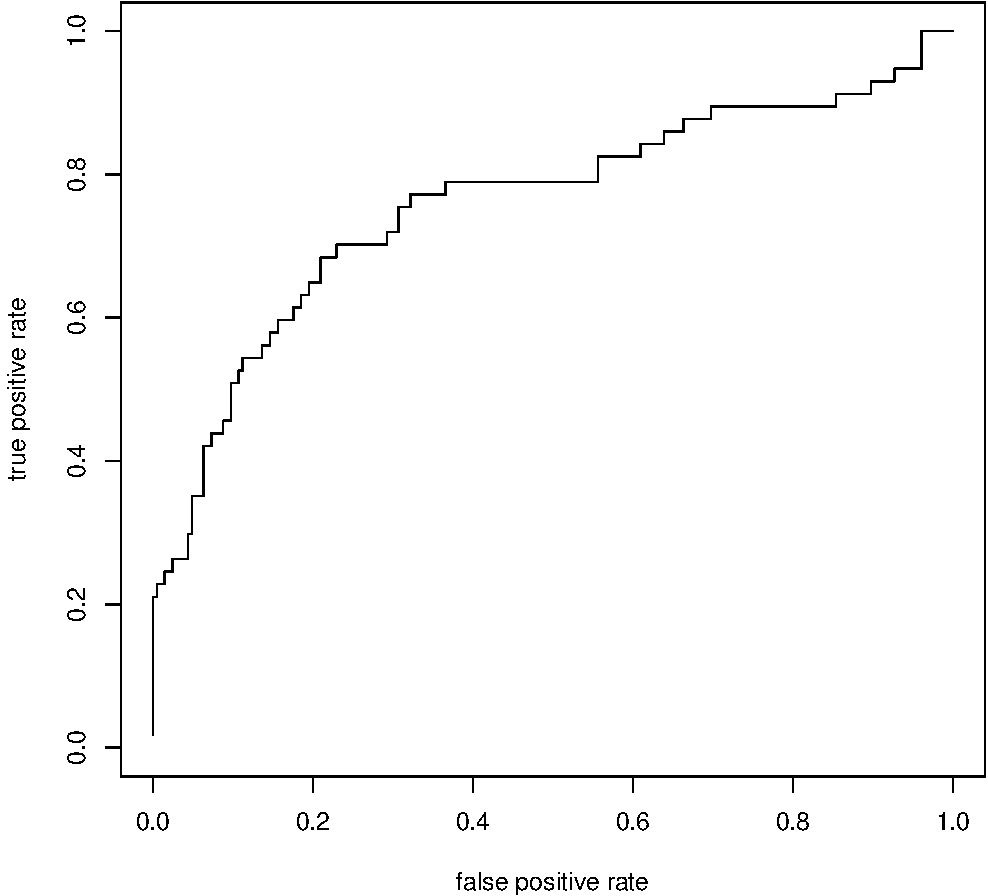
\includegraphics[width=\textwidth]{pic/ROC_DS1_1000_025.pdf}
\end{minipage}
\begin{minipage}[b]{0.45\linewidth}
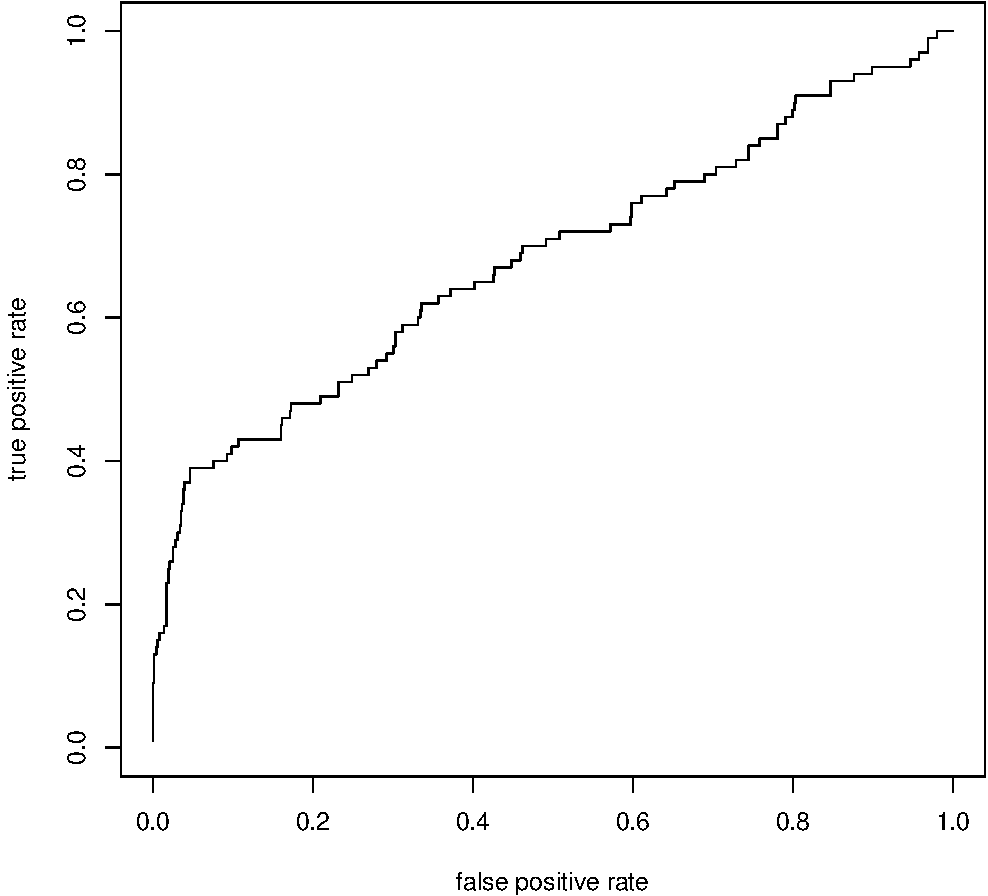
\includegraphics[width=\textwidth]{pic/ROC_DS2_1000_025.pdf}
\end{minipage}
\caption{ ROC curve using leave-one-out cross validation}
\label{fig:ROC}
\end{figure}

We also use leave-one-out cross validation to plot ROC curve and validate our model. Currently we have three sets of data: data set \#0 is the preliminary data obtained from biochemistry literature and has 36 data points; data set \#1 contains 258 data points evaluated in the first round of experiments using our algorithm; data set \#2 has 580 data points evaluated in the second round of experiments. In Figure \ref{fig:ROC}, we compare the performance of our model using different combinations of data sets, and observe that ROC curve to the left is better than the one to the right. We think that this is because data set \#2 was generated by our algorithm based on the previous two data sets, and due to the exploration manner of our algorithm, data set \#2 should lie in the region that is more challenging for the classifier. Thus it is reasonable that our classifer performs worse using all three data sets. 

\section{Optimization Algorithm}
\eqref{eq:opt} is a combinatorial optimization problem with huge feasible region. This problem is hard for any known algorithm that solves it quickly. We propose an approximation algorithm, which solves \eqref{eq:opt} using greedy heuristic, that is, starting with the empty set $S=\emptyset$, iteratively find element $e$ such that 
\begin{equation} \label{eq:greedy}
  \underset{e \in E \backslash S}{\mathrm{arg}\max} \,g(S \cup \{e\}),
\end{equation}
and incorporate it into $S$ until $|S|=K$ for some chosen K. This approach reduces the size of search space dramatically from $|E|^{|S|}$ down to $|E| \times |S|$, and we prove that if objective function $g$ is either $\PI$ or $\EI$, the proposed greedy algorithm is guaranteed to be near-optimal with a lower bound. Additionally, we show that under the statistical model described in section \ref{sec:stat model}, we can formulate \eqref{eq:greedy} as Mixed-Integer Nonlinear Programming
(MINLP). We plan to use an off-the-shelf MINLP solver to solve this problem.

\subsection{Performance guarantee for the greedy algorithm}
In this subsection, we show that when the objective function $g$ in \eqref{eq:greedy} is either $\PI$ or $\EI$, the proposed greedy algorithm has performance guarantee. The result is stated in the following:
\begin{theorem} 
If objective function is probability of improvement (i.e $\PI(S)$) or expected improvement (i.e $\EI(S)$), the greedy algorithm is guaranteed to achieve a factor $(1-1/e) (\approx 63\%)$ of the optimal value.
\end{theorem}
We prove the theorem using the following three lemmas. Lemma 1 is a result from the analysis of greedy heuristic in combinatorial optimization by Nemhauser, which provides lower bound of greedy heuristic given that objective function satisfies certain conditions. Lemma 2 and 3 show $\PI$ and $\EI$ are the objective functions that satisfy conditions stated in Lemma 1, and thus greedy algorithm has a lower bound.
\begin{lemma} \citep{Company1978}
If $F(S)$ is submodular, nondecreasing and $F(\emptyset)=0$, the greedy heuristic always produces a solution whose value is at least $1-[(K-1)/K]^K$ times the optimal value, where $|S| \leq K$. This bound can be achieved for each $K$ and has a limiting value of $1-1/e$, where $e$ is the base of the natural logarithm.
\end{lemma}

\begin{lemma} 
  Probability of improvement $\PI(S)$ is submodular, nondecreasing and $\PI(\emptyset)=0$.
\end{lemma}
\begin{lemma}
  Expected improvement $\EI(S)$ is submodular, nondecreasing and $\EI(\emptyset)=0$.
\end{lemma}

\begin{proof}[Proof of Theorem 1.]
From Lemma 2 and 3, we know that $\PI$ and $\EI$ are submodular, nondecreasing and their measure of the empty set is 0. From Lemma 1, we conclude that if the objective function $g$ in \eqref{eq:greedy} is $\PI$ or $\EI$, the greedy algorithm is guaranteed to achieve a factor of $(1-1/e)$ of the optimal value. \qedhere
\end{proof}

The proofs of Lemma 2 and 3 are available in the appendix.

\subsection{Probability of Improvement}
Since the objective function in \eqref{eq:greedy} does not have an intuitive look and is expensive to compute directly when $|S|$ is large, We show in Proposition 1 and 2 that \eqref{eq:greedy} can be written into the form in which the objective function can be easily computed using any statitical classifier. This is the general form of greedy algorithm for optimization over probability of improvement and can be used with any underlying statistical model. In addition, using the formulation in Proposition 1 and 2, we show that, under the Naive Bayes model proposed in section \ref{sec:stat model}, we can further formulate \eqref{eq:greedy} as a MINLP, and we plan to use an off-the-shelf MINLP solver to solve that.
\begin{proposition}
  If the objective function $g$ is $\PI$, we can write \eqref{eq:greedy} as 
  \begin{equation} \label{eq:PI3}
    \underset{e \in E \backslash S, f(e)<b}{\mathrm{arg}\max} \, \mathbb{P}(y(e)=1|y(x)=0, \forall x \in S).
  \end{equation}
\end{proposition}

The proof is available in the appendix. In our motivating application, using the Bayesian classification model described in section \ref{sec:stat model}, we can formulate \eqref{eq:PI3} as a MINLP. First we write equation \eqref{eq:model} as
\begin{equation} \label{model1}
\Prob\left(Y(x) = 1 | \theta\right) =
\frac{\prod_j \eta_j(x_j)}{\prod_j \eta_j(x_j) + \frac{\Prob(Y(x)=0)}{\Prob(Y(x)=1)}},
\end{equation}
where
\begin{equation*}
\eta_j(x_j) = \frac{\theta_{1,j}(x_j)}{\theta_{0,j}(x_j)} \text{\,\,\,for $\forall j \in \{1,\ldots,L\}$}. 
\end{equation*}
Then we can write equation \eqref{eq:PI3} as
\begin{equation} \label{eq:PI4}
\underset{e \in E \backslash S, f(e)<b}{\mathrm{arg}\max} \, \frac{\prod_j \eta_j(e_j)}{\prod_j \eta_j(e_j) + \frac{\Prob(Y(e)=0)}{\Prob(Y(e)=1)}},
\end{equation}
where 
\begin{equation*}
\eta_j(e_j)=\frac{\Prob(e_j|Y(e)=1,Y(x)=0, \forall x \in S)}{\Prob(e_j|Y(e)=0,Y(x)=0, \forall x \in S)}.
\end{equation*}
Now we can formulate equation \eqref{eq:PI4} as a MINLP,
\begin{equation} \label{eq:PI5}
\begin{split}
\max \quad &\frac{\prod_j \Sigma_k x_j(k) \eta_j(k)}{\prod_j \Sigma_k x_j(k) \eta_j(k) + \frac{\Prob(Y(x)=0)}{\Prob(Y(x)=1)}} \\
\text{s.t} \quad &k \in \{1,\ldots,K\} \\
&x_j(k) \in \{0,1\}\\
&\Sigma_k x_j(k)=1,
\end{split}
\end{equation}
where
\begin{equation*}
x_j(k)=\begin{dcases}
        1 & \text{if $e_j=k$}\\
        0 & \text{else}.
\end{dcases}
\end{equation*}
We summarize the algorithm in the appendix.


\subsection{Expected Improvement}
The formulation for expected improvement is similar to probability of improvement, and for our application, we can also formulate \eqref{eq:greedy} as a MINLP.
\begin{proposition}
  If the objective function $g$ is $\EI$, we can write \eqref{eq:greedy} as 
  \begin{equation} \label{eq:EI1}
    \underset{e \in E \backslash S}{\mathrm{arg}\max} \, c_0 \mathbb{P}_0(e)(b-f(e))^+ + \sum_{i=1}^{|S|} c_i \mathbb{P}_i(e)(f(x_i)-f(e))^+,
  \end{equation}
  where
  \begin{equation*}
    \begin{split}
      &\mathbb{P}_0(e)=\mathbb{P}(y(e)=1|y(x)=0, \forall x \in S), \\
      &\mathbb{P}_i(e)=\mathbb{P}(y(e)=1|y(x_i)=1, y(x_j)=0, \forall j<i, x_i,x_j \in S),
    \end{split}
  \end{equation*}
  and $c_i (i=0,\ldots,|S|)$ are known coefficients.
\end{proposition}

The proof is availabel in the appendix. Note that each term in the summation of \eqref{eq:EI1} has a similar structure as \eqref{eq:PI3}. Let $S=\{p^1,\ldots,p^{|S|}\}$, we can write \eqref{eq:EI1} as a MINLP:
\begin{equation} \label{eq:EI5}
\begin{split}
\max \quad &\Sigma_{i=0}^{|S|} c_i \frac{\prod_j \Sigma_k x_j(k) \eta_j^i(k)}{\prod_j \Sigma_k x_j(k) \eta_j^i(k) + \frac{\Prob(Y(x)=0)}{\Prob(Y(x)=1)}} (f_i-f(e))^+ \\
\text{s.t} \quad &k \in \{1,\ldots,K\} \\
&x_j(k) \in \{0,1\}\\
&\Sigma_k x_j(k)=1,
\end{split}
\end{equation}
where
\begin{equation*}
x_j(k)=\begin{dcases}
        1 & \text{if $e_j=k$}\\
        0 & \text{else},
\end{dcases}
\end{equation*}
\begin{equation*}
f_i=\begin{dcases}
        b & \text{if $i=0$}\\
        f(p^i)  & \text{else},
\end{dcases}
\end{equation*}
and $c_i$'s are known coefficients. We summarize the algorithm in the appendix.

\begin{remark}
Comparing the objective functions in \eqref{eq:PI3} and \eqref{eq:EI1}, you will notice that computation of $\PI$ is a lot cheaper than computing $\EI$, and thus solving optimization problem with $\PI$ is a lot easier than solving $\EI$, which you can observe by comparing \eqref{eq:PI5} and \eqref{eq:EI5}. However, the trade-off is that, $\PI$ only finds hits with length shorter than some threshold, whereas $\EI$ aims to optimize over length direcly and will find hits with minimal lengths. Both methods have their own advantages in achieving the goal.
\end{remark}


\section{Model Validation and Performance}
In this section we evaluate the performance of our proposed optimization methods by comparing it with two benchmark methods, in simulation, and by using it in practice.  We show our algorithm helped find a peptide with the desired property that is shorter than the shortest previously known.

% The following version was shortened.
% In this section we evaluate the performance of our proposed optimization methods by comparing it with two benchmark methods introduced in Section \ref{sec:comparison methods}. We show the performance results in Section \ref{sec:performance}. In Section \ref{sec:experiment} we show our algorithm helped find a peptide with the desired property that is shorter than the shortest previous known in our application.

%\subsection{Comparison Methods} \label{sec:comparison methods}
\paragraph{Comparison Methods}
We compare our proposed algorithm to two benchmark methods that our biochemist collaborators originally considered using: one is a typical biological evolution approach, that is, mutate known peptides with positive label, and take N peptide candidates with highest predicted probability being positive for testing. We call it mutation method. The other method is to use the trained classifier to predict probability being positive for all peptides in the library, and select N most probable ones for testing. We call it ranking method. We compare their performance below. % in Section \ref{sec:performance}.

%\subsection{Simulation Results} \label{sec:performance}
\paragraph{Simulation Results with Historical Data}
The benchmark was performed on data from previously performed experiments. We use data set \#0 and \#1 to train the statistical model, and based on this model, we generate peptides for testing using our proposed algorithm and the other two comparison methods. Then we train another statistical model using data set \#0, \#1 and \#2, and we evaluate the performance of the methods using both trained models.

% We use probability that shortest peptide $x$ with $y(x)=1$ has length smaller or equal to 12 as a measure of quality, to do the benchmark, and we show the result in Figure \ref{fig:PI}.
\begin{figure}[hpt] 
\center
\begin{minipage}{0.48\linewidth}
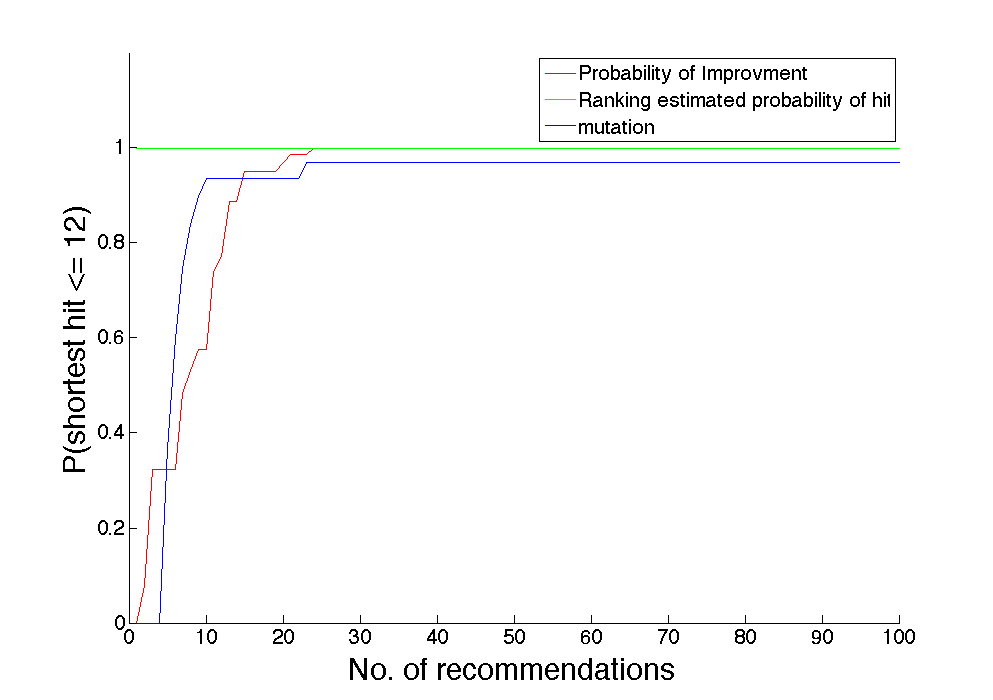
\includegraphics[width=\textwidth]{pic/PI2.png}
\end{minipage}
\begin{minipage}{0.47\linewidth}
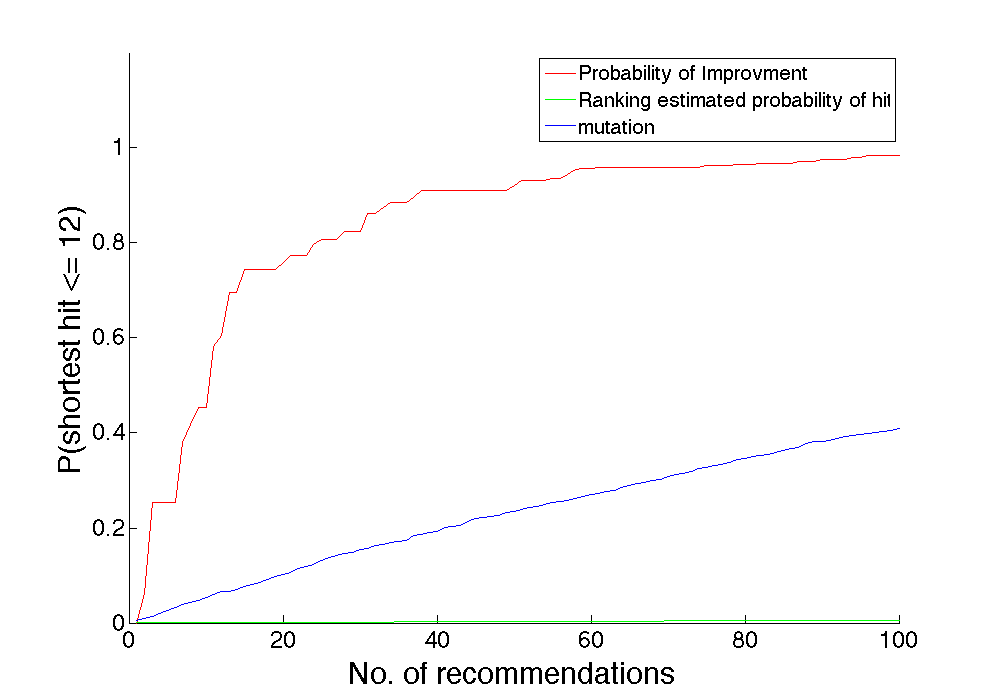
\includegraphics[width=\textwidth]{pic/PI.png}
\end{minipage}
\caption{Benchmark of Probability of Improvement algorithm}
\label{fig:PI}
\end{figure}


In Figure \ref{fig:PI} we show the benchmark using $\PI$ as performance metric. The plot to the left is calculated using the model trained on data set \#0 and \#1, and the plot to the right is obtained using the model trained on all three datasets. We notice that the performance of ranking method changes drastically across the two plots.This is because the pure exploitation behavior of ranking method makes it heavily dependent on the accuracy of underlying model. If you recall the ROC curve in Figure \ref{fig:ROC}, it shows that the statistical model is not very accurate considering limited size of training data. Since ranking method finds the ``best'' peptides based on the current model, which are  likely to be very similar to each other, in reality, if one of these peptides is not hit, then all the others are likely to be nonhits, and this is the case shown in the plot to the right. On the other hand, Probability of Improvement algorithm performs consistently well, especially in the plot to the right, where the performance is calculated using the model that the algorithm has not ``seen'', it outperforms the other two methods significantly. The reason is that the Probability of Improvement algorithm is designed to make the best decisions given the model is not perfect and tends to explore the space while generating probable hits. The diversity of the recommendation set generated by this algorithm ensures its good performance even when the underlying model is not good.

We also plan to show the benchmark using $\EI$ as performance metric in the furture.

%\subsection{Performance on Real Experiments} \label{sec:experiment}
\paragraph{Performance in Practice} \label{sec:experiment}
Given the preliminary data, we have performed two rounds of experiments using recommendations generated by Probability of Improvement algorithm. We show the histogram of length distribution of peptide hits in Figure \ref{fig:experiment} and explain how the algorithm worked to find a shorter peptide hit than the shortest peptide previously known: Ybbr sequence. Observe that all the new peptide hits found have length less than 20, this is because we set the target length $b = 20$ for our algorithm, which made the algorithm only generate peptide candidates with length less than 20. We did not set target length as the shortest length previously known, because we only have 2 short peptides from the preliminary data set and all the others have length greater than 40. Our goal for the first two rounds of experiments was to find a number of reasonably short peptide hits. After one round of experiment, we found additional 38 peptide hits, with most of them having length 19 and a few short peptides. This is expected because we have more information of long peptides than that of short peptides from the preliminary data set. To generate the second round of recommendations, we trained the statistical model using both preliminary data set and data from the first round of experiment, which contain more information on the short peptides, and we hoped to get more short peptide hits. As expected, after the second round of experiment, we can see from the histogram that there are many more short peptide hits found in this round, and we even found a peptide hit with length 10, which is shorter than ybbR sequence! We conclude that Probability of Improvement algorithm did a great job in finding short desired peptides.

\begin{figure}[hpt] 
\center
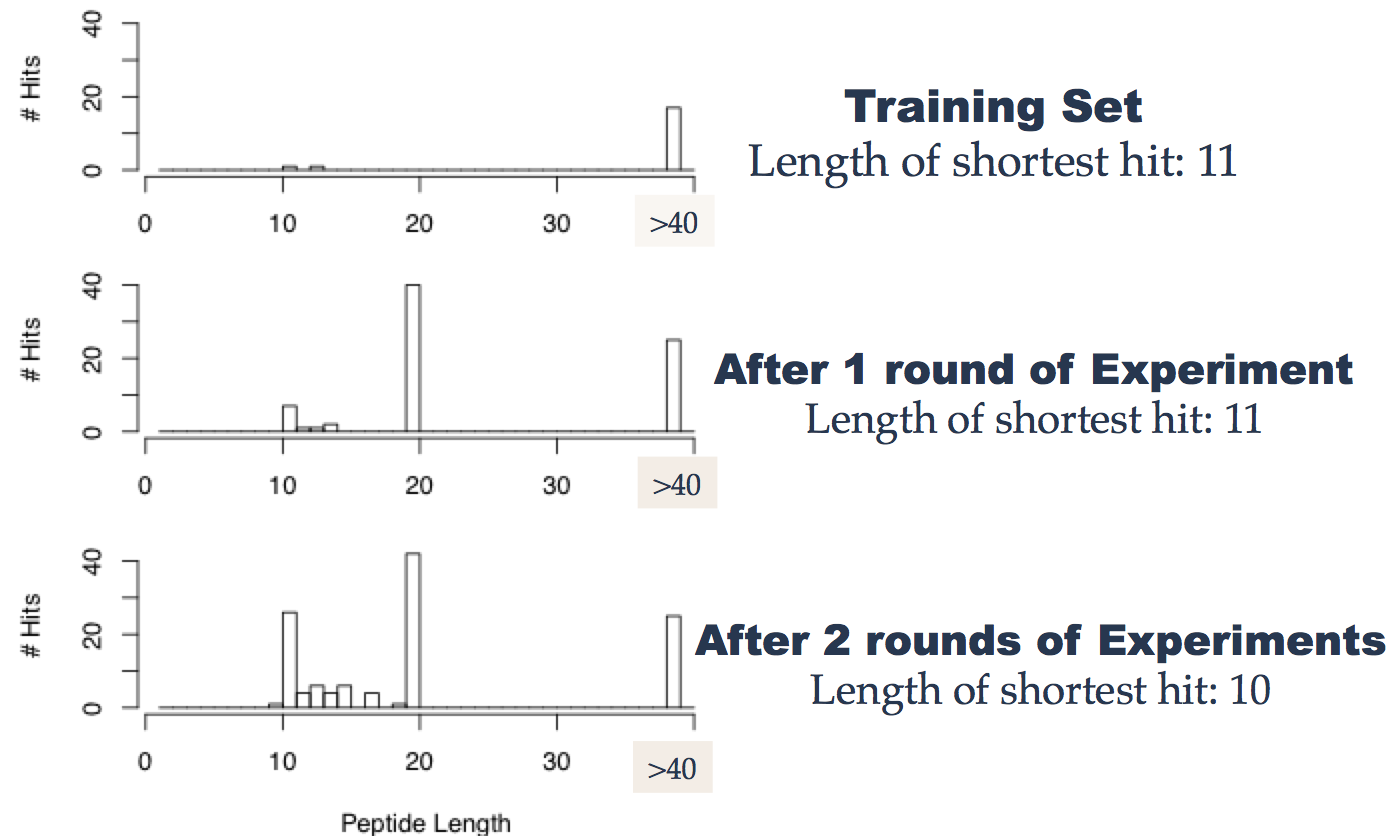
\includegraphics[width=0.6\textwidth]{pic/experiment.png}
\caption{Length distribution of target peptides.}
\label{fig:experiment}
\end{figure}


\section{Conclusion}
We proposed an optimal search algorithm based on greedy heuristic for solving the active learning problem motivated by finding short peptide substrates problem, and proved that the proposed algorithm guarantees to achieve at least a factor (1-1/e) of the optimal value. From benchmark results, we further showed that the proposed algorithm outperformed the other two heuristic search methods. In addition to theoretical results, we demonstrated effectiveness of our method in practice: so far we have performed two rounds of evaluations by doing experiments. The first round of experiments tested 258 peptides recommended by our algorithm, which is based on the statistical classifier trained using 36 preliminary data points, and the experiments took about 2 weeks to complete. As demonstrated in Figure \ref{fig:experiment}, we found 43 new peptide hits with shortest length 11 (in which 40 were obtained from baseline method, i.e. mutating existing hits, and 3 were obtained from our proposed algorithm). A month later, the second round of experiments tested 580 peptides and took another 2 weeks, in which we found another 42 new hits and a peptide hit with length 10, which is shorter than the shortest previously known (18 were obtained from mutating known hits, and 24, including the shortest hit, were obtained from our proposed algorithm). 

\section*{Appendix A: Algorithms}

\begin{Algorithm}(Probability of Improvement) \label{algo1}
\begin{algorithmic}[1]
\REQUIRE Inputs $\text{M, J, K}$, data set D and prior distribution of $\theta_y \sim \text{Dirichlet} (\boldsymbol \alpha_y), y \in \{1,0\}$
\STATE $S \leftarrow \emptyset $
\STATE Calculate posterior distribution of $\theta_1 \sim \text{Dirichlet} (\boldsymbol \alpha_1|\{x|x \in D,y(x)=1\})$.
\FOR{$m=1$ to $M$} 
\STATE COUNT $\leftarrow 0$
\STATE Calculate posterior distribution of $\theta_0 \sim \text{Dirichlet} (\boldsymbol \alpha_0|\{x|x \in D,y(x)=0\} \cup S)$.
\LOOP 
\STATE Sample $\theta_1$ from $\text{Dirichlet} (\boldsymbol \alpha_1|\{x|x \in D,y(x)=1\})$ and $\theta_0$ from $\text{Dirichlet} (\boldsymbol \alpha_0|\{x|x \in D,y(x)=0\} \cup S)$.
\STATE $\eta \leftarrow \frac{\theta_1}{\theta_0}$
\STATE Solve MINLP in equation \eqref{eq:PI5} to find $x$.
\STATE COUNT $\leftarrow$ COUNT $+ x$.
\ENDLOOP
\FOR {$j=1$ to $J$}
\STATE $e_j \leftarrow \underset{k \in \{1,\ldots,K\}}{\mathrm{arg}\max} \, \text{COUNT}_{kj}$
\ENDFOR
\STATE $S \leftarrow (S, e)$
\ENDFOR
\end{algorithmic}
\end{Algorithm}

\begin{Algorithm}(Expected Improvement) \label{algo2}
\begin{algorithmic}[1]
\REQUIRE Inputs $\text{M, J, K}$, data set D and prior distribution of $\theta_y \sim \text{Dirichlet} (\boldsymbol \alpha_y), y \in \{1,0\}$
\STATE $S \leftarrow \emptyset $
\FOR{$m=1$ to $M$} 
\STATE COUNT $\leftarrow 0$
\IF{$S$ is not empty}
\STATE Sort elements in $S$ as $\{p^1,\ldots,p^{|S|}\}$ such that $f(p^i) \leq f(p^j), \forall i<j$.
\ENDIF
\STATE Calculate posterior distribution of $\theta_1^0 \sim \text{Dirichlet} (\boldsymbol \alpha_1|\{x|x \in D,y(x)=1\})$ and $\theta_0^0 \sim \text{Dirichlet} (\boldsymbol \alpha_0|\{x|x \in D,y(x)=0\} \cup S)$.
\FOR{$i=1$ to $|S|$}
\STATE Calculate posterior distribution of $\theta_1^i \sim \text{Dirichlet} (\boldsymbol \alpha_1|\{x|x \in D,y(x)=1\} \cup \{p^i\})$ and $\theta_0^i \sim \text{Dirichlet} (\boldsymbol \alpha_0|\{x|x \in D,y(x)=0\} \cup \{p^j|j<i\})$.
\ENDFOR
\LOOP 
\STATE Sample $\theta_1^{i=0:|S|}$ and $\theta_0^{i=0:|S|}$ from posterior distribution.
\STATE $\eta^{i=0:|S|} \leftarrow \frac{\theta_1^{i=0:|S|}}{\theta_0^{i=0:|S|}}$
\STATE Solve MINLP in equation \eqref{eq:EI5} to find $x$.
\STATE COUNT $\leftarrow$ COUNT $+ x$.
\ENDLOOP
\FOR {$j=1$ to $J$}
\STATE $e_j \leftarrow \underset{k \in \{1,\ldots,K\}}{\mathrm{arg}\max} \, \text{COUNT}_{kj}$
\ENDFOR
\STATE $S \leftarrow (S, e)$
\ENDFOR
\end{algorithmic}
\end{Algorithm}

\section*{Appendix B: Mathematical Proofs}
\begin{proof}[\bf{Proof of Lemma 2.}]
First we show $\PI(\emptyset) = 0$.
\begin{equation*}
  \PI(\emptyset) = \mathbb{P}(f^*(\emptyset)<b) = \mathbb{P}(\infty<b)=0.
\end{equation*}

To show $\PI(S)$ is nondecreasing, let $A \subseteq B \subseteq E$ where $E$ is a finite set, then
\begin{equation*}
\begin{split}
\PI(B) &= \mathbb{P}(f^*(B)<b) \\
       &= \mathbb{P}(f^*(B)<b |f^*(A) \geq b) \mathbb{P}(f^*(A) \geq b) + \mathbb{P}(f^*(B)<b |f^*(A)<b) \mathbb{P}(f^*(A)<b) \\
       &= \mathbb{P}(f^*(B)<b |f^*(A) \geq b) \mathbb{P}(f^*(A) \geq b) + \mathbb{P}(f^*(A)<b) \\
       &\geq \mathbb{P}(f^*(A)<b) \\
       &= \PI(A)
\end{split}
\end{equation*}

Lastly, we want to show $\PI(S)$ is submodular. For $e \in E\backslash B$,
\begin{equation*}
\begin{split}
&\PI(A \cup \{e\}) - \PI(A) \\
&= \mathbb{P}(f^*(A \cup \{e\})<b)-\mathbb{P}(f^*(A)<b)\\
&= \mathbb{P}(f^*(A \cup \{e\})<b|f^*(A)<b)\mathbb{P}(f^*(A)<b) + \mathbb{P}(f^*(A \cup \{e\})<b|f^*(A)\geq b)\mathbb{P}(f^*(A)\geq b) -\mathbb{P}(f^*(A)<b) \\
&=\mathbb{P}(f^*(A)<b) + \mathbb{P}(f^*(A \cup \{e\})<b|f^*(A)\geq b)\mathbb{P}(f^*(A)\geq b) -\mathbb{P}(f^*(A)<b)\\
&= \mathbb{P}(f^*(A \cup \{e\})<b|f^*(A)\geq b)\mathbb{P}(f^*(A)\geq b) \\
&= \mathbb{P}(f(e)<b, y(e)=1|f^*(A)\geq b)\mathbb{P}(f^*(A)\geq b) \\
&= \mathbb{P}(f(e)<b, y(e)=1,f^*(A)\geq b)
\end{split}
\end{equation*}
Using similar argument,
\begin{equation*}
\begin{split}
&\PI(B \cup \{e\}) - \PI(B) \\
&= \mathbb{P}(f(e)<b, y(e)=1,f^*(B)\geq b) \\
&= \mathbb{P}(f(e)<b, y(e)=1,f^*(A)\geq b, f^*(B\backslash A) \geq b )
\end{split}
\end{equation*}
Therefore, $\PI(A \cup \{e\}) - \PI(A) \geq \PI(B \cup \{e\}) - \PI(B)$, thus $\PI(S)$ is submodular. \qedhere
\end{proof}


\begin{proof}[\bf{Proof of Lemma 3.}]
First we show $\EI(\emptyset) = 0$.
\begin{equation*}
  \EI(\emptyset) = \E[(b-f^*(\emptyset))^+] = \E[0] = 0.
\end{equation*}

To show $\EI(S)$ is nondecreasing, let $A \subseteq B \subseteq E$ where $E$ is a finite set. Since $f^*(B) \leq f^*(A)$, $b-f^*(B) \geq b-f^*(A)$, and $(b-f^*(B))^+ \geq (b-f^*(A))^+$, therefore, $\E[(b-f^*(B))^+] \geq \E[(b-f^*(A))^+]$.

Lastly, we want to show $\PI(S)$ is submodular. For $e \in E\backslash B$, consider $\E[(b-f^*(A \cup \{e\}))^+]-\E[(b-f^*(A))^+]$. We can write
\begin{equation*}
(b-f^*(A \cup \{e\}))^+ = \begin{dcases}
                         (b-f^*(A))^+ & \text{if $y(e)=0$} \\
                         (b-\min\{f(e),f^*(A)\})^+ & \text{if $y(e)=1$}
                         \end{dcases}
\end{equation*}
Then 
\begin{align*}
&\E[(b-f^*(A \cup \{e\}))^+]-\E[(b-f^*(A))^+] \\
&= \mathbb{P}(y(e)=1) \E[(b-\min\{f(e),f^*(A)\})^+ -(b-f^*(A))^+|y(e)=1]\\
&= \mathbb{P}(y(e)=1) \mathbb{P}(f(e)<f^*(A)|y(e)=1) \E[(b-e)^+-(b-f^*(A))^+|y(e)=1, f(e)<f^*(A)]\\
&= \E[ \mathbbm{1}_{y(e)=1, f(e)<f^*(A)} ((b-e)^+-(b-f^*(A))^+)]
\end{align*}
Since $f^*(A) \geq f^*(B)$, $\mathbbm{1}_{y(e)=1, f(e)<f^*(A)} ((b-e)^+-(b-f^*(A))^+)) \geq \mathbbm{1}_{y(e)=1, f(e)<f^*(B)} ((b-e)^+-(b-f^*(B))^+))$, thus
\begin{equation*}
\EI(A\cup \{e\})-\EI(A) \geq \EI(B\cup \{e\})-\EI(B)
\end{equation*}
$\EI(S)$ is submodular. 
\end{proof}

\begin{proof}[\bf{Proof of proposition 1.}]
  \begin{equation*}
    \begin{split}
      &\PI(S \cup \{e\}) = \mathbb{P}(f^*(S\cup \{e\})<b)\\
      &= \mathbb{P}(f^*(S)<b) + \mathbb{P}(f^*(S)\geq b) \mathbb{P}(f(e)<b, y(e)=1|f^*(S)\geq b),
    \end{split}
  \end{equation*}
  so \eqref{eq:greedy} becomes
  \begin{equation} \label{eq:PI1} 
    \underset{e \in E \backslash S}{\max} \, \PI(S \cup \{e\}) = \underset{e \in E \backslash S}{\max} \, \mathbb{P}(f(e)<b, y(e)=1|f^*(S)\geq b).
  \end{equation}
  Note that when $f(e) \geq b$, $\mathbb{P}(f(e)<b, y(e)=1|f^*(S)\geq b)=0$, thus our algorithm will always propose $e$ such that $f(e)<b$. Therefore, it is reasonable to assume that $f(x)<b$ for $\forall x \in S$, and $f^*(S)\geq b$ is equivalent to $y(x)=0$ for $\forall x \in S$. Now we can write \eqref{eq:PI1} as 
  \begin{equation*}
    \underset{e \in E \backslash S, f(e) < b}{\max} \, \mathbb{P} (y(e) = 1 \mid y(x) = 0, \forall x \in S). 
  \end{equation*}
\end{proof}

\begin{proof}[\bf{Proof of proposition 2.}]
Since choosing $e$ such that $f(e) \geq b$ has no contribution to the objective function, by using similar argument as dealing with probability of improvement, we argue that $f(x)<b$ for $\forall x \in S$. Thus
\begin{equation*}
f^*(S)  \begin{dcases}
         =\infty & \text{if $y(x)=0$ for $\forall x \in S$},\\
         < b & \text{else}.
 \end{dcases}
\end{equation*}
Now objective function we want to maximize becomes
\begin{equation*}
  \begin{split}
    &\E \left[ (b-f^*(S \cup \{e\}))^+ \right] \\
    &= \E[(b-f(e))^+ \mathbbm{1}_{f^*(S)=\infty, y(e)=1}]+ \E[ (b-f^*(S \cup \{e\}))^+ \mathbbm{1}_{f^*(S)<b}] \\
    &= \E[(b-f(e))^+ \mathbbm{1}_{f^*(S)=\infty, y(e)=1}]+ \E[ (b-f^*(S)) \mathbbm{1}_{f^*(S)<b}] + \E[(f^*(S)-f(e)) \mathbbm{1}_{y(e)=1, f(e)<f^*(S)<b}].
  \end{split}
\end{equation*}
so
\begin{equation} \label{eq:EI2}
  \begin{split}
    &\underset{e \in E \backslash S}{\max} \, \E \left[ (b-f^*(S \cup \{e\}))^+ \right], \\
    &= \underset{e \in E \backslash S, f(e)<b}{\max} \, \E[(b-f(e)) \mathbbm{1}_{f^*(S)=\infty, y(e)=1}]+\E[(f^*(S)-f(e)) \mathbbm{1}_{y(e)=1, f(e)<f^*(S)<b}].
  \end{split}
\end{equation}
For $e \in E \backslash S, f(e)<b$,
\begin{equation}
    \E[(b-f(e)) \mathbbm{1}_{f^*(S)=\infty, y(e)=1}] = \mathbb{P}(y(e)=1, y(x)=0, \forall x \in S)(b-f(e)), 
  \label{eq:EI3}
\end{equation}
\begin{equation*}
  \begin{split}
    &\E[(f^*(S)-f(e)) \mathbbm{1}_{y(e)=1, f(e)<f^*(S)<b}], \\
    &=\E[\E[(f^*(S)-f(e)) \mathbbm{1}_{y(e)=1, f(e)<f^*(S)<b}]|f^*(S)=l], \\
    &= \sum_{l \in L, f(e)<l} \mathbb{P}(y(e)=1|f^*(S)=l)(l-f(e))\mathbb{P}(f^*(S)=l),\\
  \end{split}
\end{equation*}
where $L = \{f(x): x \in S\}$. If we rank elements in $S$ such that $f(x_i) \leq f(x_j), \forall i<j, x_i,x_j \in S$, we can write equation above as
\begin{equation}
  \sum_{i=1}^{|S|} \mathbb{P}(y(e)=1, y(x_i)=1, y(x_j)=0, \forall j<i, x_i,x_j \in S)(f(x_i)-f(e))^+.
  \label{eq:EI4}
\end{equation}
Substitute \eqref{eq:EI3} \eqref{eq:EI4} into \eqref{eq:EI2}, and note that $\mathbb{P}(y(e)=1, \mathcal{F}(x_1,\ldots,x_{|S|}) \propto \mathbb{P}(y(e)=1| \mathcal{F}(x_1,\ldots,x_{|S|})$ with known coefficient given $S$, we get \eqref{eq:EI1} in proposition 2. 
\end{proof}

\section*{Appendix C: Finding Orthogonal Labeling Peptides}
An extension to the current application is to find \it{orthogonal} peptides selectively labeled by PPTases and unlabeled by AcpH, where \it{orthogonal} means a peptide can only be labeled by a specific PPTase, and be unlabeled by AcpH. Currently we investigate two kinds of PPTases: sfp and AcpS, and we look for two types of orthogonal peptides: type 1 can only be labeled by sfp and unlabeled by AcpH, while type 2 can only be labeled by AcpS and unlabeled by AcpH.

For this problem we use the similar statistical learning model as described in \ref{sec:stat model}. We originally proposed to directly use \eqref{eq:model}, and simply redefine $Y(x)=1$ as peptide $x$ is type 1 or type 2. This is simple, as all the previous developed algorithms apply to the new application, and the only thing we need to do is to modify the training dataset according to the new definitions of ``labeling''. However, we have 580 peptides from earlier experiments only tested using sfp and AcpH, and we cannot use these precious experimental data for training since we do not have their labeling property about AcpS. 

We tweaked the original idea and proposed a new method: for a peptide $x$, we define three types of labeling, where $Y_1(x) = 1$ means $x$ can be labeled by sfp, $Y_2(x)$ means $x$ can be labeled by AcpS, and $Y_3(x)$ means given $x$ is labeled, $x$ can be unlabeled by AcpH. Now
\begin{equation*}
\begin{split}
\mathbb{P} (\text{$x$ is type 1}) &=\mathbb{P} (Y_1(x) = 1, Y_2(x) = 0, \text{$x$ can be unlabeled by AcpH}),\\
&= \mathbb{P} (Y_1(x) = 1, Y_2(x) = 0) \mathbb{P} (Y_3(x)), \\
&= \mathbb{P} (Y_1(x) = 1) \mathbb{P} (Y_2(x) = 0) \mathbb{P} (Y_3(x) = 1),
\end{split}
\end{equation*}
and similarly,
\begin{equation*}
\mathbb{P} (\text{$x$ is type 2}) = \mathbb{P} (Y_1(x) = 0) \mathbb{P} (Y_2(x) = 1) \mathbb{P} (Y_3(x) = 1).
\end{equation*}
Thus we can create three datasets and use \eqref{eq:model} to train three seperate models. Since prediction on labeling property for sfp does not depend on the labeling property for AcpS, we can utilize the 580 data points for training on both labeling by sfp and unlabeling by AcpH, which were left out by original training method.

However, for the new method, we need to tweak our optimization algorithm in \eqref{eq:PI5} and \eqref{eq:EI5}, which will be updated later.
% Acknowledgments here
% \acknowledgment{The authors gratefully acknowledge the existence of
% the Journal of Irreproducible Results and the support of the Society
% for the Preservation of Inane Research.}
\bibliography{DataMiningPaper}
\bibliographystyle{plainnat}
%%%%%%%%%%%%%%%%%
\end{document}
%%%%%%%%%%%%%%%%%
